\documentclass[twoside]{book}

% Packages required by doxygen
\usepackage{fixltx2e}
\usepackage{calc}
\usepackage{doxygen}
\usepackage[export]{adjustbox} % also loads graphicx
\usepackage{graphicx}
\usepackage[utf8]{inputenc}
\usepackage{makeidx}
\usepackage{multicol}
\usepackage{multirow}
\PassOptionsToPackage{warn}{textcomp}
\usepackage{textcomp}
\usepackage[nointegrals]{wasysym}
\usepackage[table]{xcolor}

% Font selection
\usepackage[T1]{fontenc}
\usepackage[scaled=.90]{helvet}
\usepackage{courier}
\usepackage{amssymb}
\usepackage{sectsty}
\renewcommand{\familydefault}{\sfdefault}
\allsectionsfont{%
  \fontseries{bc}\selectfont%
  \color{darkgray}%
}
\renewcommand{\DoxyLabelFont}{%
  \fontseries{bc}\selectfont%
  \color{darkgray}%
}
\newcommand{\+}{\discretionary{\mbox{\scriptsize$\hookleftarrow$}}{}{}}

% Page & text layout
\usepackage{geometry}
\geometry{%
  a4paper,%
  top=2.5cm,%
  bottom=2.5cm,%
  left=2.5cm,%
  right=2.5cm%
}
\tolerance=750
\hfuzz=15pt
\hbadness=750
\setlength{\emergencystretch}{15pt}
\setlength{\parindent}{0cm}
\setlength{\parskip}{3ex plus 2ex minus 2ex}
\makeatletter
\renewcommand{\paragraph}{%
  \@startsection{paragraph}{4}{0ex}{-1.0ex}{1.0ex}{%
    \normalfont\normalsize\bfseries\SS@parafont%
  }%
}
\renewcommand{\subparagraph}{%
  \@startsection{subparagraph}{5}{0ex}{-1.0ex}{1.0ex}{%
    \normalfont\normalsize\bfseries\SS@subparafont%
  }%
}
\makeatother

% Headers & footers
\usepackage{fancyhdr}
\pagestyle{fancyplain}
\fancyhead[LE]{\fancyplain{}{\bfseries\thepage}}
\fancyhead[CE]{\fancyplain{}{}}
\fancyhead[RE]{\fancyplain{}{\bfseries\leftmark}}
\fancyhead[LO]{\fancyplain{}{\bfseries\rightmark}}
\fancyhead[CO]{\fancyplain{}{}}
\fancyhead[RO]{\fancyplain{}{\bfseries\thepage}}
\fancyfoot[LE]{\fancyplain{}{}}
\fancyfoot[CE]{\fancyplain{}{}}
\fancyfoot[RE]{\fancyplain{}{\bfseries\scriptsize Generated by Doxygen }}
\fancyfoot[LO]{\fancyplain{}{\bfseries\scriptsize Generated by Doxygen }}
\fancyfoot[CO]{\fancyplain{}{}}
\fancyfoot[RO]{\fancyplain{}{}}
\renewcommand{\footrulewidth}{0.4pt}
\renewcommand{\chaptermark}[1]{%
  \markboth{#1}{}%
}
\renewcommand{\sectionmark}[1]{%
  \markright{\thesection\ #1}%
}

% Indices & bibliography
\usepackage{natbib}
\usepackage[titles]{tocloft}
\setcounter{tocdepth}{3}
\setcounter{secnumdepth}{5}
\makeindex

% Custom commands
\newcommand{\clearemptydoublepage}{%
  \newpage{\pagestyle{empty}\cleardoublepage}%
}

\usepackage{caption}
\captionsetup{labelsep=space,justification=centering,font={bf},singlelinecheck=off,skip=4pt,position=top}

%===== C O N T E N T S =====

\begin{document}

% Titlepage & ToC
\pagenumbering{alph}
\begin{titlepage}
\vspace*{7cm}
\begin{center}%
{\Large My Project }\\
\vspace*{1cm}
{\large Generated by Doxygen 1.8.14}\\
\end{center}
\end{titlepage}
\clearemptydoublepage
\pagenumbering{roman}
\tableofcontents
\clearemptydoublepage
\pagenumbering{arabic}

%--- Begin generated contents ---
\chapter{File Index}
\section{File List}
Here is a list of all files with brief descriptions\+:\begin{DoxyCompactList}
\item\contentsline{section}{\textbf{ main.\+c} }{\pageref{main_8c}}{}
\end{DoxyCompactList}

\chapter{File Documentation}
\section{main.\+c File Reference}
\label{main_8c}\index{main.\+c@{main.\+c}}
{\ttfamily \#include $<$stdio.\+h$>$}\newline
{\ttfamily \#include $<$stdlib.\+h$>$}\newline
{\ttfamily \#include $<$math.\+h$>$}\newline
{\ttfamily \#include $<$time.\+h$>$}\newline
Include dependency graph for main.\+c\+:
\nopagebreak
\begin{figure}[H]
\begin{center}
\leavevmode
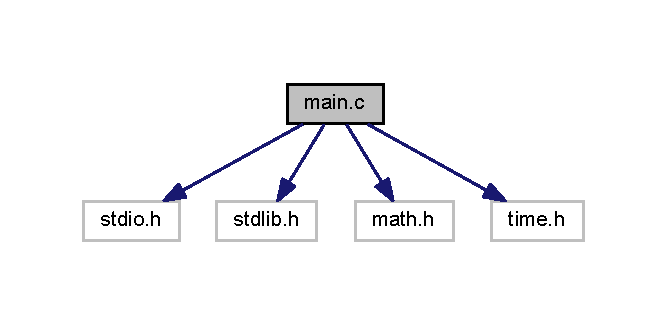
\includegraphics[width=320pt]{main_8c__incl}
\end{center}
\end{figure}
\subsection*{Macros}
\begin{DoxyCompactItemize}
\item 
\#define \textbf{ max}(a,  b)~( ((a) $>$ (b)) ? (a) \+: (b) )
\end{DoxyCompactItemize}
\subsection*{Functions}
\begin{DoxyCompactItemize}
\item 
int \textbf{ Tai\+Teava} (int \textbf{ n}, int P\+R\+ET[$\,$])
\item 
int \textbf{ main} ()
\end{DoxyCompactItemize}
\subsection*{Variables}
\begin{DoxyCompactItemize}
\item 
int \textbf{ n}
\item 
int \textbf{ i}
\item 
int \textbf{ j}
\item 
int \textbf{ Pret\+Maxim}
\end{DoxyCompactItemize}


\subsection{Macro Definition Documentation}
\mbox{\label{main_8c_affe776513b24d84b39af8ab0930fef7f}} 
\index{main.\+c@{main.\+c}!max@{max}}
\index{max@{max}!main.\+c@{main.\+c}}
\subsubsection{max}
{\footnotesize\ttfamily \#define max(\begin{DoxyParamCaption}\item[{}]{a,  }\item[{}]{b }\end{DoxyParamCaption})~( ((a) $>$ (b)) ? (a) \+: (b) )}



Definition at line 7 of file main.\+c.



\subsection{Function Documentation}
\mbox{\label{main_8c_ae66f6b31b5ad750f1fe042a706a4e3d4}} 
\index{main.\+c@{main.\+c}!main@{main}}
\index{main@{main}!main.\+c@{main.\+c}}
\subsubsection{main()}
{\footnotesize\ttfamily int main (\begin{DoxyParamCaption}{ }\end{DoxyParamCaption})}



Definition at line 34 of file main.\+c.

Here is the call graph for this function\+:
\nopagebreak
\begin{figure}[H]
\begin{center}
\leavevmode
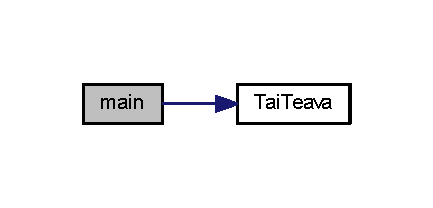
\includegraphics[width=208pt]{main_8c_ae66f6b31b5ad750f1fe042a706a4e3d4_cgraph}
\end{center}
\end{figure}
\mbox{\label{main_8c_a716c4869232d48f9b77f6a715ffe0df0}} 
\index{main.\+c@{main.\+c}!Tai\+Teava@{Tai\+Teava}}
\index{Tai\+Teava@{Tai\+Teava}!main.\+c@{main.\+c}}
\subsubsection{Tai\+Teava()}
{\footnotesize\ttfamily int Tai\+Teava (\begin{DoxyParamCaption}\item[{int}]{n,  }\item[{int}]{P\+R\+ET[$\,$] }\end{DoxyParamCaption})}



Definition at line 15 of file main.\+c.

Here is the caller graph for this function\+:
\nopagebreak
\begin{figure}[H]
\begin{center}
\leavevmode
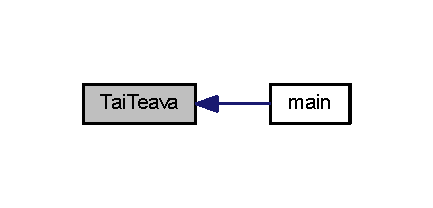
\includegraphics[width=208pt]{main_8c_a716c4869232d48f9b77f6a715ffe0df0_icgraph}
\end{center}
\end{figure}


\subsection{Variable Documentation}
\mbox{\label{main_8c_acb559820d9ca11295b4500f179ef6392}} 
\index{main.\+c@{main.\+c}!i@{i}}
\index{i@{i}!main.\+c@{main.\+c}}
\subsubsection{i}
{\footnotesize\ttfamily int i}



Definition at line 12 of file main.\+c.

\mbox{\label{main_8c_a37d972ae0b47b9099e30983131d31916}} 
\index{main.\+c@{main.\+c}!j@{j}}
\index{j@{j}!main.\+c@{main.\+c}}
\subsubsection{j}
{\footnotesize\ttfamily int j}



Definition at line 12 of file main.\+c.

\mbox{\label{main_8c_a76f11d9a0a47b94f72c2d0e77fb32240}} 
\index{main.\+c@{main.\+c}!n@{n}}
\index{n@{n}!main.\+c@{main.\+c}}
\subsubsection{n}
{\footnotesize\ttfamily int n}



Definition at line 12 of file main.\+c.

\mbox{\label{main_8c_ac3eb8db17fea6f06278fb25ab78664ac}} 
\index{main.\+c@{main.\+c}!Pret\+Maxim@{Pret\+Maxim}}
\index{Pret\+Maxim@{Pret\+Maxim}!main.\+c@{main.\+c}}
\subsubsection{Pret\+Maxim}
{\footnotesize\ttfamily int Pret\+Maxim}



Definition at line 13 of file main.\+c.


%--- End generated contents ---

% Index
\backmatter
\newpage
\phantomsection
\clearemptydoublepage
\addcontentsline{toc}{chapter}{Index}
\printindex

\end{document}
